\section{PlanesQML}

The last of the 3 Qt based GUIs is PlanesQML. This uses QML, a declarative language similar to html to create the graphical interfaces.

\subsection{Main Window}

The main.cpp for the project looks as follows:

\begin{lstlisting}
	QGuiApplication app(argc, argv);
	QQmlApplicationEngine engine;
	
	PlaneGameQML planeGame;
	PlaneGridQML player_pgq(&planeGame, planeGame.playerGrid());
	PlaneGridQML computer_pgq(&planeGame, planeGame.computerGrid());
	player_pgq.initGrid();
	computer_pgq.initGrid();
	
	engine.rootContext()->setContextProperty("PlayerPlaneGrid", &player_pgq);
	engine.rootContext()->setContextProperty("ComputerPlaneGrid", &computer_pgq);
	engine.rootContext()->setContextProperty("PlaneGame", &planeGame);
	engine.load(QUrl(QStringLiteral("qrc:/main.qml")));
\end{lstlisting}

The QML interpreting engine is define by an object of the type QQmlApplicationEngine. Our application implements everything in QML except for the game engine, which is implemented in C++. In order to be able to reference the C++ objects in QML, two wrapper classes were created: PlaneGameQML and PlaneGridQML. 

Here below is the header file for PlaneGameQML:

\begin{lstlisting}

class PlaneGameQML : public QObject
{
	Q_OBJECT
public:
	PlaneGameQML();
	~PlaneGameQML();

public:
	Q_INVOKABLE void doneEditing();
	Q_INVOKABLE inline int getPlayerMoves() { return m_Stats.m_playerMoves; }
	Q_INVOKABLE inline int getPlayerHits() { return m_Stats.m_playerHits; }
	Q_INVOKABLE inline int getPlayerDead() { return m_Stats.m_playerDead; }
	Q_INVOKABLE inline int getPlayerMisses() { return m_Stats.m_playerMisses; }
	Q_INVOKABLE inline int getPlayerWins() { return m_Stats.m_playerWins; }
	Q_INVOKABLE inline int getComputerMoves() { return m_Stats.m_computerMoves; }
	Q_INVOKABLE inline int getComputerHits() { return m_Stats.m_computerHits; }
	Q_INVOKABLE inline int getComputerDead() { return m_Stats.m_computerDead; }
	Q_INVOKABLE inline int getComputerMisses() { return m_Stats.m_computerMisses; }
	Q_INVOKABLE inline int getComputerWins() { return m_Stats.m_computerWins; }
	
	Q_INVOKABLE void startNewGame();
	
	inline PlaneGrid* playerGrid() { return mRound->playerGrid(); }
	inline PlaneGrid* computerGrid() { return mRound->computerGrid(); }

signals:
	void guessMade(const GuessPoint& gp);
	void computerMoveGenerated(const GuessPoint& gp);    
	void updateStats();
	void roundEnds(bool isPlayerWinner);
	void resetGrid();

public slots:
	void statsUpdated(const GameStatistics& stats);
	void receivedPlayerGuess(const GuessPoint& gp);

private:
	//The controller object
	PlaneRound* mRound;
	GameStatistics m_Stats;
};

\end{lstlisting}

Observe that the class derives from QObject and that some methodes are declared using the Qt macro Q\_INVOKABLE. This allows the methods to be accessible from the QML code. PlaneGridQML has a header file with the same characteristics.

In order to register the C++ object with the QML engine one uses the setContextProperty() function as shown above.

By using the function load() one can define the start qml object for the project: main.qml

\begin{lstlisting}

Window {
	visible: true
	width: 1000
	height: 700

Row {
	anchors.fill: parent
	LeftPane {
		id: leftPane
	}
	RightPane {
		id: rightPane
	}
	}
}
\end{lstlisting}

This defines a window with 100 X 700 size composed of two subobjects: LeftPane and RightPane, which play similar roles as in PlanesGraphicsScene.

\begin{figure}[h]
	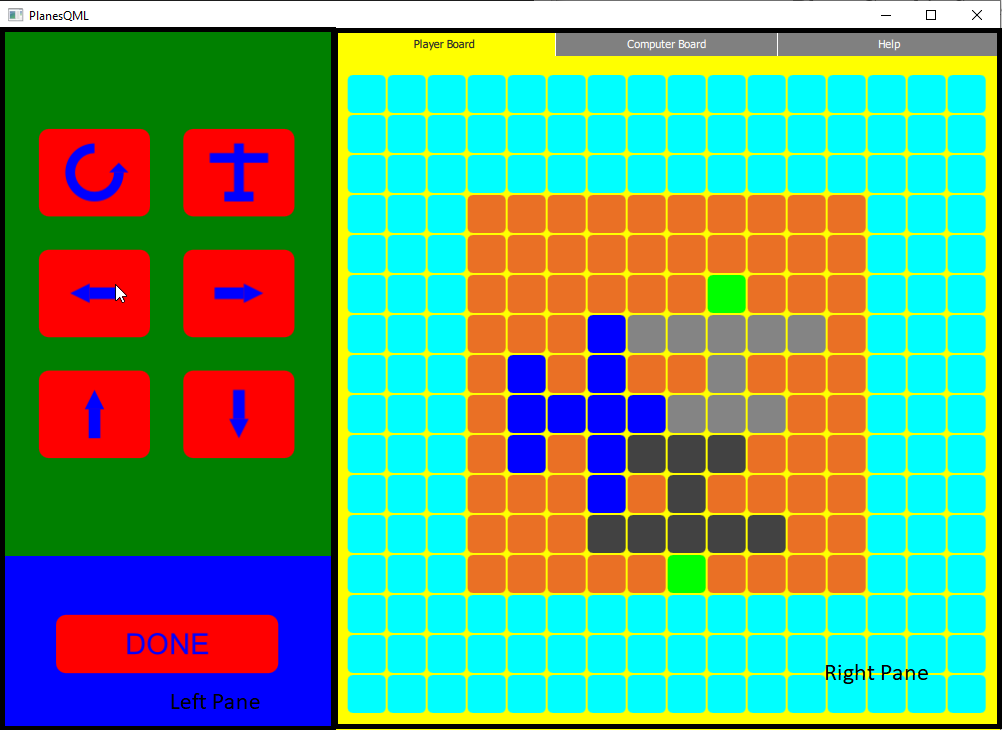
\includegraphics[width = \textwidth]{PlanesQML_BoardEditing_WidgetNames.png}
	\caption{Simplified Layout of PlanesQML}
	\label{fig:planesqml_boardediting_widgetnames}
\end{figure}

\subsection {LeftPane}

The QML code for the left pane is as follows:

\begin{lstlisting}
Rectangle {
	width: parent.width/3
	height: parent.height
	property alias currentTab : stack.currentIndex
	
	StackLayout {
		id: stack
		width: parent.width
		height: parent.height
		
		currentIndex: 1
		GameStatistics {
			id: roundTab
		}
		BoardEditorControls {
		}
		Rectangle {
			id: startTab
			color: "blue"
		}
	}
	
	Connections {
		target: PlaneGame
		onUpdateStats: {
			roundTab.playerMoves = PlaneGame.getPlayerMoves()
			roundTab.playerHits = PlaneGame.getPlayerHits()
			roundTab.playerMisses = PlaneGame.getPlayerMisses()
			roundTab.playerDead = PlaneGame.getPlayerDead()
			roundTab.playerWins = PlaneGame.getPlayerWins()
			roundTab.computerMoves = PlaneGame.getComputerMoves()
			roundTab.computerHits = PlaneGame.getComputerHits()
			roundTab.computerMisses = PlaneGame.getComputerMisses()
			roundTab.computerDead = PlaneGame.getComputerDead()
			roundTab.computerWins = PlaneGame.getComputerWins()
		}
	}
}
\end{lstlisting}

It contains a start tab, a board editing tab, containing the buttons to position the planes board, and a game tab, displaying computer and player game statistics during the game. These objects are grouped under a stack layout, that is a widget containing more superimposed widgets. For an explanation of the Connections element see \ref{qml:connections}.

\subsubsection {BoardEditing Tab}

The board editing tab contains buttons to position the planes on the game board. Here below is the implementation for the plane rotation button.


\begin{lstlisting}
import "ButtonPaintFunctions.js" as PaintFunctions

Rectangle {
	id: back
	color: "red"
	radius: 10
	
	Canvas {
		width: back.width
		height: back.height
		
		onPaint: {
			var ctx = getContext("2d")
			PaintFunctions.rotateButton(ctx)
		}
	}
	
	MouseArea {
		width: parent.width
		height: parent.height
		onClicked: {
		//console.log("Rotate clicked")
		anim.start()
		PlayerPlaneGrid.rotateSelectedPlane();
		PlayerPlaneGrid.verifyPlanePositionValid()
		}
	}
	
	SequentialAnimation {
		id: anim
		PropertyAnimation { target: back; property: "color"; to: "green"; duration: 50 }
		PropertyAnimation { target: back; property: "color"; to: "red"; duration: 50 }
		}
}
\end{lstlisting}

The button is encapsulated inside a rectangle with rounded corners (see attribute radius of the QML object Rectangle). It contains a canvas element which defines the design of the button. This is accomplished in the signal handler onPaint. In order to react to click events a MouseArea element is used. To graphically represent the click event a small animation is created - see \ref{qml:animation}.

One remarks here that the buttons are not standard buttons as for example the Qt Widgets buttons that we used in PlanesWidgets or PlanesGraphicScene. They are completely custom defined, proving the flexibility and resourcefullness of QML.

\subsubsection {Game Tab}

\subsubsection {Start New Game Tab}

\subsection {QML Concepts}

\subsubsection {QML Objects}

QML objects can be declared with the following syntax: 

\begin{lstlisting}

ObjectTypeName {

	attribute1: value1
	attribute2: value2
	..................
}

\end{lstlisting}

One such example is the main window object:

\begin{lstlisting}

Window {
	visible: true
	width: 1000
	height: 700
}

\end{lstlisting}

\subsubsection {QML Object property}
\subsubsection {QML Object property aliases}
\subsubsection {QML Subobjects}

In a QML application a hierarchy of objects and sub-objects exists. This hierarchy has a single root object. In our case it is the main window object. The other objects are all sub-objects of this main object. 
For example LeftPane and RightPane are sub-objects of the main window. 

\subsubsection {QML Layouts}

One type of QML objects are layouts. For example Row in the main window allows to display the LeftPane and RightPane in the same horizontal row. Other examples of layouts used in this application are: StackLayout (used in the LeftPane), ColumnLayout and GridLayout (used in GameStatistics)

\subsubsection {QML GridView}

\subsubsection {QML ListView}

\subsubsection {QML Canvas}

\subsubsection {QML Animations} \label{qml:animation}

In the definition of the rotation button, we see the following code block:

\begin{lstlisting}
SequentialAnimation {
	id: anim
	PropertyAnimation { target: back; property: "color"; to: "green"; duration: 50 }
	PropertyAnimation { target: back; property: "color"; to: "red"; duration: 50 }
}
\end{lstlisting}

Here a sequence of two animations is defined. Each of the two is a so called PropertyAnimation, where a property of a QML object changes over time. In this particular case, the property color of the object named back is to change to green over 50 ms, the first animation, and the property color of the object named back is to be then changed to red over the same duration of 50 ms.


\subsubsection {QML MouseArea} \label{qml:mouse_area}

The MouseArea element is used to capture events from the mouse. We illustrate this with the code of the MovePlaneDownwards button, used for board editing.

\begin{lstlisting}
Rectangle {
	id: back
	color: "red"
	radius: 10
	
	Canvas {
		anchors.fill: parent
		width: back.width
		height: back.height
		
		onPaint: {
			var ctx = getContext("2d")
			PaintFunctions.moveDownButton(ctx)
		}
	}
	
	MouseArea {
		width: parent.width
		height: parent.height
		onClicked: {
			//console.log("Plane downwards clicked")
			anim.start()
			PlayerPlaneGrid.moveDownSelectedPlane()
			PlayerPlaneGrid.verifyPlanePositionValid()
		}
	}
	
	SequentialAnimation {
		id: anim
		PropertyAnimation { target: back; property: "color"; to: "green"; duration: 50 }
		PropertyAnimation { target: back; property: "color"; to: "red"; duration: 50 }
	}
}
\end{lstlisting}

In the MouseArea, a onClicled element is defined, which describes what is be done when one clicks in the region associated with MouseArea.
The surface covered by the MouseArea is defined with the help of the width and height attributes, in this case they are as big as the containing button.

\subsubsection {QML States}

Here below is a part of the listing of the done button, used to confirm when the user has finished positioning his planes on the game board. 

\begin{lstlisting}
Rectangle {
	id: back
	state: "Enabled"
	
	Connections {
		target: PlayerPlaneGrid
		onPlanePositionNotValid: {
		if (val == true) {
		back.state = "Disabled"
		//console.log("Plane position not valid")
		} else {
		back.state = "Enabled"
		//console.log("Plane position valid")
		}
		}
	}
	
	states: [
		State {
			name: "Enabled"
			PropertyChanges {
				target: back
				color: back.enabledColor
		}
		},
		State {
			name: "Disabled"
			PropertyChanges {
				target: back
				color: back.disabledColor
			}
		}
	]
}

\end{lstlisting}

In the states attribute the possible states of the button are defined: Enabled and Disabled. When switching to theses states the background color of the button changes to enabledColor when Enabled and to disabledColor when Disabled.

\subsubsection {QML Connections Attribute} \label{qml:connections}

In the definition of the LeftPane we see the following block:

\begin{lstlisting}
Connections {
target: PlaneGame
onUpdateStats: {
	roundTab.playerMoves = PlaneGame.getPlayerMoves()
	roundTab.playerHits = PlaneGame.getPlayerHits()
	roundTab.playerMisses = PlaneGame.getPlayerMisses()
	roundTab.playerDead = PlaneGame.getPlayerDead()
	roundTab.playerWins = PlaneGame.getPlayerWins()
	roundTab.computerMoves = PlaneGame.getComputerMoves()
	roundTab.computerHits = PlaneGame.getComputerHits()
	roundTab.computerMisses = PlaneGame.getComputerMisses()
	roundTab.computerDead = PlaneGame.getComputerDead()
	roundTab.computerWins = PlaneGame.getComputerWins()
	}
}
	
\end{lstlisting}

In this case this code block allows to connect to a signal from a C++ object, registered with the QML engine with the name PlaneGame. 
This is an extension of the normal version of reacting to signals from QML objects presented in the section \ref{qml:mouse_area}.